\chapter*{Part B\@: Autoencoders}

\section*{Introduction}

This part of the assignment aims to implement an autoencoder on the full MNIST
dataset.

\section*{Stacked Denoising Autoencoder}

The stacked denoising autoencoder consists of three hidden layers with 900, 625
and 400 neurons respectively. The following plot shows the training cost of the
autoencoder.

\begin{center}
    \includegraphics[width=\imgw]{project_2b_ae/train}
\end{center}

The following images show 100 samples of weights learned at each layer.

\begin{longtabu}{X[c]X[c]}
    \includegraphics[width=\imgwt]{project_2b_ae/weight1} &
    \includegraphics[width=\imgwt]{project_2b_ae/weight2} \\
    \includegraphics[width=\imgwt]{project_2b_ae/weight3}
\end{longtabu}

100 test images are chosen at random; the images and their reconstructions are
shown below.

\begin{longtabu}{X[c]X[c]}
    \includegraphics[width=\imgwt]{project_2b_ae/input} &
    \includegraphics[width=\imgwt]{project_2b_ae/output}
\end{longtabu}

The hidden layer activations are shown below.

\begin{longtabu}{X[c]X[c]}
    \includegraphics[width=\imgwt]{project_2b_ae/layer1} &
    \includegraphics[width=\imgwt]{project_2b_ae/layer2} \\
    \includegraphics[width=\imgwt]{project_2b_ae/layer3}
\end{longtabu}

\section*{Feedforward Neural Network on Autoencoder}

We added a softmax and an output layer to the stacked denoising autoencoder
described above, to make a classifier on MNIST data. The training cost is shown 
below.

\begin{center}
    \includegraphics[width=\imgw]{project_2b_ae/train_ffn}
\end{center}

The test accuracy is shown below; the classifier achieves 97.2\% accuracy after
25 epochs.

\begin{center}
    \includegraphics[width=\imgw]{project_2b_ae/test_ffn}
\end{center}

\section*{Autoencoder with Momentum and Sparsity}

We added the momentum term and sparsity into the autoencoder. The following plot
shows the training cost of the autoencoder.

\begin{center}
    \includegraphics[width=\imgw]{project_2b_ae_sparsity/train}
\end{center}

The following images show 100 samples of weights learned at each layer.

\begin{longtabu}{X[c]X[c]}
    \includegraphics[width=\imgwt]{project_2b_ae_sparsity/weight1} &
    \includegraphics[width=\imgwt]{project_2b_ae_sparsity/weight2} \\
    \includegraphics[width=\imgwt]{project_2b_ae_sparsity/weight3}
\end{longtabu}

The same 100 images and their reconstructions are shown below.

\begin{longtabu}{X[c]X[c]}
    \includegraphics[width=\imgwt]{project_2b_ae_sparsity/input} &
    \includegraphics[width=\imgwt]{project_2b_ae_sparsity/output}
\end{longtabu}

The hidden layer activations are shown below.

\begin{longtabu}{X[c]X[c]}
    \includegraphics[width=\imgwt]{project_2b_ae_sparsity/layer1} &
    \includegraphics[width=\imgwt]{project_2b_ae_sparsity/layer2} \\
    \includegraphics[width=\imgwt]{project_2b_ae_sparsity/layer3}
\end{longtabu}

The training cost of the autoencoder classifier on MNIST data is shown below.

\begin{center}
    \includegraphics[width=\imgw]{project_2b_ae_sparsity/train_ffn}
\end{center}

The test accuracy is shown below; the classifier achieves 97.3\% accuracy
after 25 epochs.

\begin{center}
    \includegraphics[width=\imgw]{project_2b_ae_sparsity/test_ffn}
\end{center}